\chapter{Modelo de datos}
En este anexo vamos a utilizar un diagrama para mostrar como se encuentra la estructura del sistema a nivel de base de datos. 
También se especifica el código de colores se utiliza para identificar diferentes tipos de entidades.

\section{Código de colores y atributos}

El código de colores permite identificar el tipo de información que guarda una entidad o tabla:


\begin{itemize}
    \item \IUEntidaB{} Este color se utiliza para representar entidades relacionadas al negocio.
    \item \IUEntidaA{} Este color se utiliza para representar entidades de tipo catálogo es decir, tiene información definida 
    y que no puede ser alterada por medio del sistema.
    \item \IUEntidaC{} Este color se utiliza para representar entidades de tipo catálogo editable es decir, tiene información definida 
    y que puede ser alterada por medio del sistema.
    \item \IUEntidaD{} Este color se utiliza para representar entidades de tipo estado.
\end{itemize}

Cada dato que nos interese de una entidad se coloca en forma de atributo, acompañado de su respectiva descripción y tipo de dato. Con ello, se busca indicar la naturaleza del atributo y restringir sus valores posibles. Entre los tipos de dato más comunes, encontramos los siguientes:

    \begin{bGlosario}
	\bTerm{tBool}{bool}
	    Valor booleano, es decir, toma únicamente los valores 0 y 1.

        \bTerm{tInt}{int}
            Solo valores enteros, incluido el 0
            
        \bTerm{tNumeric}{numeric} (precisión, escala)
            Número cuyo número de dígitos está indicado por precisión, de los cuales
            los definidos en escala son a la izquierda del punto y el resto a la derecha.
            
        \bTerm{tChar}{Char}
            Cadena de caracteres de la longitud indicada, si se guarda una cadena de menor
            tamaño, los caracteres no utilizados serán espacios en blanco.
            
        \bTerm{tVarchar}{varchar} (longitud)
            Cadena de caracteres de longitud variable. 
        \bTerm{tEmail}{email} (longitud)
            
        \bTerm{tDate}{date} Fecha
        \bTerm{tTime}{time} Hora
    \end{bGlosario}

Cada dato puede tener restricciones adicionales, entre las que se encuentran:
    
    \begin{bGlosario}
    
        \bTerm{tRequerido}{Requerido}
            Indica que el dato es obligatorio y no puede existir un registro sin que éste tenga
            un valor.
            
        \bTerm{tUnico}{Único}
            Indica que los valores para un atributo o combinación de estos no se deben
            repetir en los diferentes registros.
            
        \bTerm{tDefault}{default}
            Permite especificar un valor por defecto para el atributo.
            
        \bTerm{tPrimaryKey}{primary key}
            Indica el atributo o combinación de éstos que serán la llave primaria. La llave
            primaria es el identificador único de cada registro dentro de la tabla, por lo
            que debe ser requerido y único.
            
        \bTerm{tForeignKey}{Foreign key}
            Indica el atributo o conjunto de éstos que son llave foránea y apuntan a otra
            tabla, esto es, sus valores posibles solo pueden ser aquellos que existan en la
            llave primaria a la que apuntan. FK(Tabla.atributo).

            
    \end{bGlosario}
    

\section{Diagrama Relacional}

En la figura \textbf{ref} se muestra el diagrama de datos con base en el análisis de requerimientos que
del \textbf{ref} y los  casos de uso que se presentan en el \textbf{ref}
%\begin{figure}[hbtp!]
%5    \begin{center}
%           % \includegraphics[width=.65\textwidth]{negocio/images/MI-POA-CH}
%            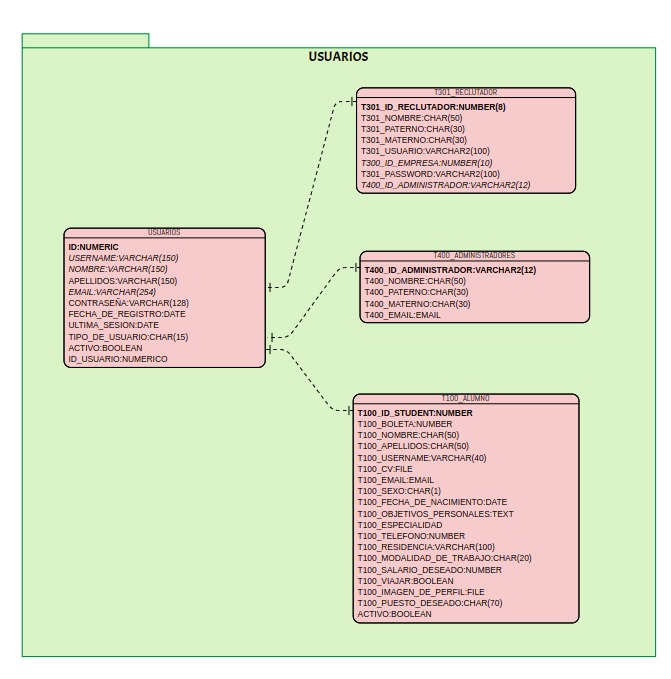
\includegraphics[width=.6\textwidth]{anexos/imagenes/Usuarios.jpeg}
%            
%    \end{center}
%        \label{fig:MI-Planeacion}
%            \caption{Diagrama de base de datos del módulo de Usuarios}
%    
%    \end{figure}

% En la figura  \ref{fig:MI-PlaneacionI}
%\begin{figure}[hbtp!]
%    \begin{center}
%        \includegraphics[width=.7\textwidth]{negocio/images/MI-POA-CAT}
%    \end{center}
%    \label{fig:MI-PlaneacionI}
%\end{figure}
%
%\begin{figure}[hbtp!]
%    \begin{center}
%        \includegraphics[width=.7\textwidth]{negocio/images/MI-POA-CFG}
%    \end{center}
%    \label{fig:MI-PlaneacionII}
%\end{figure}
%
%\begin{figure}[hbtp!]
%    \begin{center}
%        \includegraphics[width=.7\textwidth]{negocio/images/MI-POA-PLA}
%    \end{center}
%    \label{fig:MI-PlaneacionIII}
%\end{figure}

%---------------------Usuario-----------------------------
\begin{cdtEntidad}{users}{Usuario}{
        Esta entidad es generada por Django. 
    }
	    \brAttr{id}{Id de usuario}{tInt}{
	        Identificador único para cada registro de la entidad usuarios.
            Restricciones adicionales:
            \begin{Citemize}
                \item \refElem{tPrimaryKey}
                \item \refElem{tUnico}
            \end{Citemize}
        }{\datRequerido}

        \brAttr{email}{Correo electrónico}{tEmail}{
	        Es el correo del alumno con el cual se identificara como unico dentro del sistema.
	        Restricciones adicionales:
            \begin{Citemize}
                \item \refElem{tUnico}
            \end{Citemize}
        }{\datRequerido}
    
        \brAttr{password}{Contraseña}{tVarchar}{
	        Es la contraseña de acceso al sistema para el usuario.
            Restricciones adicionales:
            \begin{Citemize}
                \item Debe de cumplir con el formato correcto de acuerdo a \refIdElem{RN-N006}
            \end{Citemize}
        }{\datRequerido}

        \brAttr{fecharegis}{Fecha de registro}{tDate}{
	        Es la fecha en la que el usuario crea su cuenta en el sistema y el propio sistema 
            la registra.
        }{\datRequerido}

        \brAttr{ultsesion}{Ultima sesión}{tDate}{
	        Es la fecha en la que el usuario inició sesión en el sistema (se registra automáticamente).
        }{\datRequerido}

        \brAttr{idtipo}{Id de tipo}{tNumeric}{
            Es la referencia a la entidad \refElem{users}
            Restricciones adicionales:
            \begin{Citemize}
                \item \refElem{tForeignKey}
                \item \refElem{tUnico}
            \end{Citemize}
        }{\datRequerido}

        \brAttr{status}{Activo}{tBool}{
	        Es el estado de la cuenta del usuario dentro del sistema.
        }{\datRequerido}

\end{cdtEntidad}

%---------------------Tipo Usuario-----------------------------
\begin{cdtEntidad}{tipo_users}{Usuario}{
    Esta entidad es el catalogo que indica si el tipo de usuario es un candidato, reclutador, encatgado o colaborador.
}
    \brAttr{id}{Id de usuario}{tInt}{
        Identificador único para cada registro de la entidad.
        Restricciones adicionales:
        \begin{Citemize}
            \item \refElem{tPrimaryKey}
            \item \refElem{tUnico}
        \end{Citemize}
    }{\datRequerido}

    \brAttr{descripcion}{Descripción}{tVarchar}{
        Es el nombre del tipo del usuario.
    }{\datRequerido}
\end{cdtEntidad}

%---------------------Empresa-----------------------------
\begin{cdtEntidad}{empresa}{Empresa}{
    Empresa constituida que publica vacantes en el sistema siempre y cuando lo haya permitido el 
    encargado/colaborador del sistema.
    }

    \brAttr{id}{Id de la empresa}{tInt}{
	    Identificador único para cada registro de la empresa.
        Restricciones adicionales:
        \begin{Citemize}
            \item \refElem{tPrimaryKey}
            \item \refElem{tUnico}
        \end{Citemize}
    }{\datRequerido} 

    \brAttr{nombre}{Nombre}{tVarchar}{
        Nombre de la empresa con el que se registra en el sistema.
    }{\datRequerido}

    \brAttr{rfc}{RFC}{tVarchar}{
        RFC de la empresa.
        Restricciones adicionales:
        \begin{Citemize}
            \item Debe de cumplir con la regla de negocio ...
            \item \refElem{tUnico}
        \end{Citemize}
    }{\datRequerido}

    \brAttr{dominio}{Dominio}{tVarchar}{
        Nombre de la empresa con el que se registra en el sistema.
    }{\datRequerido}

    \brAttr{razonsocial}{Razón social}{tVarchar}{
        Razon social de la empresa.
    }{\datRequerido}

    \brAttr{pageweb}{Página Web}{tVarchar}{
        Es el URL de la oágina de la empresa.
    }{\datOpcional}
    
    \brAttr{logo}{Logo}{tVarchar}{
        Imagen del logo representativo de la empresa.
    }{\datOpcional}

    \brAttr{banner}{Banner}{tVarchar}{
        Imagen secundaria del logo representativo de la empresa.
    }{\datOpcional}

    %\brAttr{mision}{Misión}{tVarchar}{Descripción}{\datOpcional}
    %\brAttr{vision}{Vision}{tVarchar}{Descripción}{\datOpcional}
    %\brAttr{fecha-alta}{Fecha de alta}{tDate}{Descripción}{\datOpcional}
    \brAttr{idEncargado}{Id del encargado del sistema}{tInt}{
	   Es el identificador que hace referencia al encargado del sistema.
	   Restricciones adicionales:
        \begin{Citemize}
            \item \refElem{tForeignKey}
            \item \refElem{tUnico}
        \end{Citemize}
    }{\datRequerido}

    \brAttr{idEstado}{Id del estado}{tInt}{
	   Es el identificador que hace referencia al estado que tiene la empresa en el sistema..
	   Restricciones adicionales:
        \begin{Citemize}
            \item \refElem{tForeignKey}
            \item \refElem{tUnico}
        \end{Citemize}
    }{\datRequerido}
\end{cdtEntidad}

%---------------------Reclutador-----------------------------
\begin{cdtEntidad}{reclutador}{Reclutador}{
    Es el personal de recursos humanos de la empresa que ya esta registrada en el sistema.}
    \brAttr{id}{Id de reclutador}{tInt}{
        Identificador único para cada registro de un reclutador.
        Restricciones adicionales:
        \begin{Citemize}
            \item \refElem{tPrimaryKey}
            \item \refElem{tUnico}
        \end{Citemize}
    }{\datRequerido} 

    \brAttr{nombre}{Nombre}{tChar}{
        Nombre del reclutador con el cual se registra en el sistema.
        Restricciones adicionales:
        \begin{Citemize}
            \item No debe de exceder de 50 caracteres.
        \end{Citemize}
    }{\datRequerido}

    \brAttr{papellido}{Primer apellido}{tChar}{
        Primer apellido del reclutador con el cual se registra en el sistema.
        Restricciones adicionales:
            \begin{Citemize}
                \item No debe de execer de 60 caracteres.
            \end{Citemize}
    }{\datRequerido}

    \brAttr{sapellido}{Segundo apellido}{tChar}{
        Segundo apellido del reclutador con el cual se registra en el sistema.
        Restricciones adicionales:
            \begin{Citemize}
                \item No debe de execer de 60 caracteres.
            \end{Citemize}
    }{\datOpcional}

    \brAttr{telefono}{Telefono}{tNumeric}{
        Número del telefono del reclutador.
        Restricciones adicionales:
            \begin{Citemize}
                \item Tiene que ser exactamente de 10 dígitos.
            \end{Citemize}
    }{\datRequerido}

    \brAttr{email}{Correo electrónico}{tEmail}{
	    Es el correo del reclutador.
	    Restricciones adicionales:
            \begin{Citemize}
                \item \refElem{tUnico}
            \end{Citemize}
    }{\datRequerido}

    \brAttr{idEmpresa}{Id}{tInt}{
        Es la referencia al id del registro de la empresa.
        Restricciones adicionales:
        \begin{Citemize}
            \item \refElem{tForeignKey}
        \end{Citemize}
    }{\datOpcional}

    \brAttr{idEstatusR}{Id}{tInt}{
        Es la referencia al id del estatus del reclutador.
        Restricciones adicionales:
        \begin{Citemize}
            \item \refElem{tForeignKey}
        \end{Citemize}
    }{\datOpcional}

    \brAttr{idEncargado}{Id}{tInt}{
        Es la referencia al id del encargado.
        Restricciones adicionales:
        \begin{Citemize}
            \item \refElem{tForeignKey}
        \end{Citemize}
    }{\datOpcional}

    %\brAttr{id-admin}{Id}{tInt}{Descripción}{\datOpcional}
\end{cdtEntidad}

%---------------------EStado del Reclutador-----------------------------
\begin{cdtEntidad}{estadoReclutador}{Estado Reclutador}{
    Esta entidad es el catalogo que indica si el estado del reclutador.
}
    \brAttr{id}{Id}{tInt}{
        Identificador único para cada registro de la entidad.
        Restricciones adicionales:
        \begin{Citemize}
            \item \refElem{tPrimaryKey}
            \item \refElem{tUnico}
        \end{Citemize}
    }{\datRequerido}

    \brAttr{descripcion}{Descripción}{tVarchar}{
        Es el nombre estado del usuario.
    }{\datRequerido}
\end{cdtEntidad}

%---------------------EStado del Empresa-----------------------------
\begin{cdtEntidad}{estadoEmpresa}{Estado Empresa}{
    Esta entidad es el catalogo que indica si el estado de la empresa.
}
    \brAttr{id}{Id}{tInt}{
        Identificador único para cada registro de la entidad.
        Restricciones adicionales:
        \begin{Citemize}
            \item \refElem{tPrimaryKey}
            \item \refElem{tUnico}
        \end{Citemize}
    }{\datRequerido}

    \brAttr{descripcion}{Descripción}{tVarchar}{
        Es el nombre estado del estado de la empresa.
    }{\datRequerido}
\end{cdtEntidad}



%---------------------Alumno-----------------------------
\begin{cdtEntidad}{candidato}{Candidato}{Un alumno es un tipo de usuario dentro del sistema.}
    \brAttr{id-alumno}{Id}{tInt}{
        Identificador único para cada registro de la entidad alumno.
            Restricciones adicionales:
            \begin{Citemize}
                \item \refElem{tPrimaryKey}
                \item \refElem{tUnico}
            \end{Citemize}
    }{\datRequerido} 

    \brAttr{boleta}{Número de boleta}{tNumeric}{
        Es el número de boleta de los alumnos del Instituto Politécnico Nacional.
            Restricciones adicionales:
            \begin{Citemize}
                \item Debe de cumplir con la regla de negocio ...
                \item \refElem{tUnico}
            \end{Citemize}
    }{\datOpcional}

    \brAttr{nombre}{Nombre}{tChar}{
        Nombre del alumno con el cual se registra en el sistema.
        Restricciones adicionales:
            \begin{Citemize}
                \item No debe de execer de 50 caracteres.
            \end{Citemize}
    }{\datRequerido}

    \brAttr{papellido}{Primer apellido}{tChar}{
        Primer apellido del alumno con el cual se registra en el sistema.
        Restricciones adicionales:
            \begin{Citemize}
                \item No debe de execer de 60 caracteres.
            \end{Citemize}
    }{\datRequerido}

    \brAttr{sapellido}{Segundo apellido}{tChar}{
        Segundo apellido del alumno con el cual se registra en el sistema.
        Restricciones adicionales:
            \begin{Citemize}
                \item No debe de execer de 60 caracteres.
            \end{Citemize}
    }{\datOpcional}

    \brAttr{pdfcv}{CV/Resume}{tVarchar}{
        Archivo en formato \textbf{.pdf} del alumno.
        Restricciones adicionales:
            \begin{Citemize}
                \item No debe de execer de 100 caracteres.
            \end{Citemize}
    }{\datOpcional}

    \brAttr{email}{Correo electrónico}{tEmail}{
	    Es el correo del alumno.
	    Restricciones adicionales:
            \begin{Citemize}
                \item \refElem{tUnico}
            \end{Citemize}
    }{\datRequerido}
    
    \brAttr{objetivospersonales}{Objetivos personales}{tVarchar}{
        Descripción de los objetivos personales del alumno.
    }{\datOpcional}
    
    \brAttr{puestodeseado}{Puesto deseado}{tChar}{
        Nombre del puesto deseado del alumno.
        Restricciones adicionales:
            \begin{Citemize}
                \item No debe de execer de 70 caracteres.
            \end{Citemize}
    }{\datOpcional}
    
    \brAttr{telefono}{Telefono}{tNumeric}{
        Número del telefono del alumno.
        Restricciones adicionales:
            \begin{Citemize}
                \item Tiene que ser exactamente de 10 dígitos.
            \end{Citemize}
    }{\datRequerido}
    
    \brAttr{recidencia}{Recidencia}{tVarchar}{
        Lugar donde se ubica el alumno.
    }{\datRequerido}

    \brAttr{salario}{Salario deseado}{tNumeric}{
        Cantidad salarial que desea percibir el alumno.
    }{\datOpcional}

    \brAttr{reubicable}{Reubicable}{tBool}{
        Indica si el alumno esta dispuesto a cambiar de lugar de recidencia o no.
    }{\datOpcional}

    \brAttr{imagenperfil}{Imagen de perfil}{tVarchar}{
        Es la imagen del perfil del alumno:
        Los tipos de archivos que se permiten son:
            \begin{Citemize}
                \item .png
                \item .jpg
                \item .jpge
            \end{Citemize}
    }{\datOpcional}

    \brAttr{status}{Activo}{tBool}{
	        Es el estado de la cuenta del usuario dentro del sistema.
    }{\datOpcional}
   
    \brAttr{modalidad}{Tipo de trabajo}{tVarchar}{
       Es el tipo de trabajo que prefiere el alumno.
       Los valores posibles son:
            \begin{Citemize}
                \item Hibrido
                \item Presencial
                \item Home oficce
            \end{Citemize}
    }{\datOpcional}

\end{cdtEntidad}
%---------------------Historial Academico-----------------------------
\begin{cdtEntidad}{hacademico}{Historial Academico}{
    Esta entidad almacena todos 
    }

    \brAttr{id}{Id}{tInt}{
        Identificador único para cada registro de la entidad.
        Restricciones adicionales:
        \begin{Citemize}
            \item \refElem{tPrimaryKey}
            \item \refElem{tUnico}
        \end{Citemize}
    }{\datRequerido}

    \brAttr{idalumno}{idalumno}{tInt}{
        Identificador único para cada registro de la entidad alumno.
            Restricciones adicionales:
            \begin{Citemize}
                \item \refElem{tForeignKey}
                \item \refElem{tUnico}
            \end{Citemize}
    }{\datRequerido} 
    
    \brAttr{idCarrera}{idCarrera}{tInt}{
        Identificador único para cada registro de la entidad.
        Restricciones adicionales:
        \begin{Citemize}
            \item \refElem{tForeignKey}
            \item \refElem{tUnico}
        \end{Citemize}
    }{\datRequerido}

    \brAttr{idUnidadAcademica}{idUnidadAcademica}{tInt}{
        Identificador único para cada registro de la entidad.
        Restricciones adicionales:
        \begin{Citemize}
            \item \refElem{tForeignKey}
            \item \refElem{tUnico}
        \end{Citemize}
    }{\datRequerido}

    \brAttr{idEstadoAcademico}{idEstadoAcademico}{tInt}{
        Identificador único para cada registro de la entidad.
        Restricciones adicionales:
        \begin{Citemize}
            \item \refElem{tForeignKey}
            \item \refElem{tUnico}
        \end{Citemize}
    }{\datRequerido}

    \brAttr{idNivelAcademico}{IdNivelAcademico}{tInt}{
        Identificador único para cada registro de la entidad.
        Restricciones adicionales:
        \begin{Citemize}
            \item \refElem{tForeignKey}
            \item \refElem{tUnico}
        \end{Citemize}
    }{\datRequerido}

    \brAttr{fechaini}{Fecha de inicio}{tDate}{
        Fecha en la que inicio el nivel academico.
    }{\datRequerido}

    \brAttr{fechafin}{Fecha final}{tDate}{
        Fecha en la que finalizó el nivel academico.
    }{\datRequerido}
\end{cdtEntidad}
%---------------------Red Social----------------------------
\begin{cdtEntidad}{RedSocial}{Red Social}{
    Esta entidad guarda todas las redes solciales qeu el candidato haya registrado en el sistema desde su perfil.
}
  \brAttr{id}{Id}{tInt}{
        Identificador único para cada registro de la entidad.
        Restricciones adicionales:
        \begin{Citemize}
            \item \refElem{tPrimaryKey}
            \item \refElem{tUnico}
        \end{Citemize}
    }{\datRequerido}

    \brAttr{idalumno}{idalumno}{tInt}{
        Identificador único para cada registro de la entidad alumno.
            Restricciones adicionales:
            \begin{Citemize}
                \item \refElem{tForeignKey}
                \item \refElem{tUnico}
            \end{Citemize}    
    }{\datRequerido}
\end{cdtEntidad}


%---------------------Nivel academico-----------------------------
\begin{cdtEntidad}{NivelAcademico}{Nivel academico}{
    Esta entidad es el catalogo que indica el nivel academico del usuario.
}
    \brAttr{id}{Id}{tInt}{
        Identificador único para cada registro de la entidad.
        Restricciones adicionales:
        \begin{Citemize}
            \item \refElem{tPrimaryKey}
            \item \refElem{tUnico}
        \end{Citemize}
    }{\datRequerido}

    \brAttr{descripcion}{Descripción}{tVarchar}{
        Es el nombre del nivel academico.
    }{\datRequerido}
\end{cdtEntidad}

%---------------------Unidad Academica-----------------------------
\begin{cdtEntidad}{UnidadAcademica}{Unidad Academica}{
    Esta entidad es el catalogo que indica la Unidad Academica a la que el usuario esta asociado.
}
    \brAttr{id}{Id}{tInt}{
        Identificador único para cada registro de la entidad.
        Restricciones adicionales:
        \begin{Citemize}
            \item \refElem{tPrimaryKey}
            \item \refElem{tUnico}
        \end{Citemize}
    }{\datRequerido}

    \brAttr{descripcion}{Descripción}{tVarchar}{
        Es el nombre de la Unidad Academica.
    }{\datRequerido}
\end{cdtEntidad}

%---------------------Estado Academico-----------------------------
\begin{cdtEntidad}{EstadoAcademico}{Estado Academico}{
    Esta entidad es el catalogo que indica el Estado Academico al que el usuario esta asociado.
}
    \brAttr{id}{Id}{tInt}{
        Identificador único para cada registro de la entidad.
        Restricciones adicionales:
        \begin{Citemize}
            \item \refElem{tPrimaryKey}
            \item \refElem{tUnico}
        \end{Citemize}
    }{\datRequerido}

    \brAttr{descripcion}{Descripción}{tVarchar}{
        Es el nombre del Estado Academico.
    }{\datRequerido}
\end{cdtEntidad}

%---------------------Carrera-----------------------------
\begin{cdtEntidad}{Carrera}{Carrera}{
    Esta entidad es el catalogo que indica la Carrera al que el usuario esta asociado.
}
    \brAttr{id}{Id}{tInt}{
        Identificador único para cada registro de la entidad.
        Restricciones adicionales:
        \begin{Citemize}
            \item \refElem{tPrimaryKey}
            \item \refElem{tUnico}
        \end{Citemize}
    }{\datRequerido}

    \brAttr{descripcion}{Descripción}{tVarchar}{
        Es el nombre de la Carrera.
    }{\datRequerido}
\end{cdtEntidad}

%---------------------Plataforma-----------------------------
\begin{cdtEntidad}{Plataforma}{Plataforma}{
    Esta entidad es el catalogo que indica la Plataforma de la red solcial que usuario tiene registrado.
}
    \brAttr{id}{Id}{tInt}{
        Identificador único para cada registro de la entidad.
        Restricciones adicionales:
        \begin{Citemize}
            \item \refElem{tPrimaryKey}
            \item \refElem{tUnico}
        \end{Citemize}
    }{\datRequerido}

    \brAttr{descripcion}{Descripción}{tVarchar}{
        Es el nombre de la Plataforma.
    }{\datRequerido}
\end{cdtEntidad}

%---------------------Vacante----------------------------
\begin{cdtEntidad}{vacante}{Vacante}{
    Vacante publicada por un reclutador de una empresa.}
    \brAttr{id}{Id}{tInt}{
        Identificador único para cada registro de cada vacante publicada en el sistema.
        Restricciones adicionales:
        \begin{Citemize}
            \item \refElem{tPrimaryKey}
            \item \refElem{tUnico}
        \end{Citemize}
    }{\datRequerido} 

    \brAttr{puesto}{Puesto}{tVarchar}{
        Texto breve el cual describe el puesto de la vacante que publica el sistema.
    }{\datRequerido}

    \brAttr{descripcion}{Descripción}{tVarchar}{
       Es la descripción de la vacante, la cual puede contener:
       \begin{Citemize}
            \item Requisitos de la vacante.
            \item Actividades que va realizar.
            \item Idiomas, habilidades y conocimientos.
        \end{Citemize}
    }{\datRequerido}

    \brAttr{ubicacion}{Localidad}{tVarchar}{
        Indica la ubicación de la vacante, siempre y cuando sea presencial o hibrida.
        Restricciones adicionales:
        \begin{Citemize}
            \item \refElem{tForeignKey}
        \end{Citemize}
    }{\datRequerido}

    \brAttr{fechap}{Fecha de publicación}{tDate}{
        Indica la fecha en la que se publico la vacante.
    }{\datRequerido}

    \brAttr{fechac}{Fecha de cierre}{tDate}{
        Indica la fecha en la que se cierra o se va cerrar la vacante, por 
        defecto la decha de cierre es un mes despues de su fecha de publicación
        si el reclutador de la vacante no lo indica.
    }{\datRequerido}

    \brAttr{salariomin}{Salario mínimo}{tNumeric}{
        Salario minimo que puede percibir el candidato a la vacante.
    }{\datOpcional}

    \brAttr{saraliomax}{Salario máximo}{tNumeric}{
        Salario máximo que puede percibir el candidato a la vacante.
    }{\datOpcional}

    \brAttr{diaslab}{Días laborales}{tVarchar}{
        Indica los días en los que el candidato debe trabajar en dado casos
        que sea contratado.
    }{\datOpcional}

    \brAttr{horaentra}{Horario de entrada}{tTime}{
        Indica la hora de entrada de trabajo de la vacante.
    }{\datOpcional}
    
    \brAttr{horasal}{Horario de salida}{tTime}{
        Indica la hora de salida de trabajo de la vacante.
    }{\datOpcional}
\end{cdtEntidad}

%---------------------EStado de la Vacante-----------------------------
\begin{cdtEntidad}{estadoVacante}{Estado Vacante}{
    Esta entidad es el catalogo que indica si el estado de la vacante.
}
    \brAttr{id}{Id}{tInt}{
        Identificador único para cada registro de la entidad.
        Restricciones adicionales:
        \begin{Citemize}
            \item \refElem{tPrimaryKey}
            \item \refElem{tUnico}
        \end{Citemize}
    }{\datRequerido}

    \brAttr{descripcion}{Descripción}{tVarchar}{
        Es el nombre estado del estado de la vacante.
    }{\datRequerido}
\end{cdtEntidad}

%---------------------EStado de la Vacante-----------------------------
\begin{cdtEntidad}{CestadoSolicitud}{Estado Solicitud}{
    Esta entidad es el catalogo que indica si el estado de la solicitud.
}
    \brAttr{id}{Id}{tInt}{
        Identificador único para cada registro de la entidad.
        Restricciones adicionales:
        \begin{Citemize}
            \item \refElem{tPrimaryKey}
            \item \refElem{tUnico}
        \end{Citemize}
    }{\datRequerido}

    \brAttr{descripcion}{Descripción}{tVarchar}{
        Es el nombre estado del estado de la solicitud.
    }{\datRequerido}
\end{cdtEntidad}


%---------------------Perfil del Candidato-----------------------------
\begin{cdtEntidad}{perfilCandidato}{Estado Solicitud}{
    Esta entidad es el catalogo que indica el tipo de perfil que tiene el candidato.
}
    \brAttr{id}{Id}{tInt}{
        Identificador único para cada registro de la entidad.
        Restricciones adicionales:
        \begin{Citemize}
            \item \refElem{tPrimaryKey}
            \item \refElem{tUnico}
        \end{Citemize}
    }{\datRequerido}

    \brAttr{descripcion}{Descripción}{tVarchar}{
        Es el nombre estado del perfil del candidato.
    }{\datRequerido}
\end{cdtEntidad}

%---------------------Perfil del Candidato-----------------------------
\begin{cdtEntidad}{perfilCandidato}{Perfil del Candidato}{
    Esta entidad es el catalogo que indica el tipo de perfil que tiene el candidato.
}
    \brAttr{id}{Id}{tInt}{
        Identificador único para cada registro de la entidad.
        Restricciones adicionales:
        \begin{Citemize}
            \item \refElem{tPrimaryKey}
            \item \refElem{tUnico}
        \end{Citemize}
    }{\datRequerido}

    \brAttr{descripcion}{Descripción}{tVarchar}{
        Es el nombre estado del perfil del candidato.
    }{\datRequerido}
\end{cdtEntidad}


%---------------------Experiencia Laboral-----------------------------
\begin{cdtEntidad}{expLaboral}{Experiencia Laboral}{
    Esta entidad es el catalogo que indica la experiencia que tiene el candidato.
}
    \brAttr{id}{Id}{tInt}{
        Identificador único para cada registro de la entidad.
        Restricciones adicionales:
        \begin{Citemize}
            \item \refElem{tPrimaryKey}
            \item \refElem{tUnico}
        \end{Citemize}
    }{\datRequerido}

    \brAttr{descripcion}{Descripción}{tVarchar}{
        Es el nombre estado del perfil del candidato.
    }{\datRequerido}
\end{cdtEntidad}

%---------------------Tipo de Contratación-----------------------------
\begin{cdtEntidad}{TipoContra}{Tipo de Contratación}{
    Esta entidad es el catalogo que indica el tipo de contratación que desea el candidato.
}
    \brAttr{id}{Id}{tInt}{
        Identificador único para cada registro de la entidad.
        Restricciones adicionales:
        \begin{Citemize}
            \item \refElem{tPrimaryKey}
            \item \refElem{tUnico}
        \end{Citemize}
    }{\datRequerido}

    \brAttr{descripcion}{Descripción}{tVarchar}{
        Es el nombre del tipo de contratación que desea el candidato.
    }{\datRequerido}
\end{cdtEntidad}

%---------------------Modalidad de Trabajo-----------------------------
\begin{cdtEntidad}{modalidadT}{Modalidad de Trabajo}{
    Esta entidad es el catalogo que indica de modalidad que desea el candidato.
}
    \brAttr{id}{Id}{tInt}{
        Identificador único para cada registro de la entidad.
        Restricciones adicionales:
        \begin{Citemize}
            \item \refElem{tPrimaryKey}
            \item \refElem{tUnico}
        \end{Citemize}
    }{\datRequerido}

    \brAttr{descripcion}{Descripción}{tVarchar}{
        Es el nombre del tipo de modalidad que desea el candidato.
    }{\datRequerido}
\end{cdtEntidad}

%---------------------Nivel-----------------------------
\begin{cdtEntidad}{nivel}{Nivel}{
    Esta entidad es el catalogo que indica del idioma que tiene el candidato.
}
    \brAttr{id}{Id}{tInt}{
        Identificador único para cada registro de la entidad.
        Restricciones adicionales:
        \begin{Citemize}
            \item \refElem{tPrimaryKey}
            \item \refElem{tUnico}
        \end{Citemize}
    }{\datRequerido}

    \brAttr{descripcion}{Descripción}{tVarchar}{
        Es el nombre que indica del idioma que tiene  el candidato.
    }{\datRequerido}
\end{cdtEntidad}

%---------------------Catalogo Idiomas-----------------------------
\begin{cdtEntidad}{catIdioma}{Catalogo Idiomas}{
    Esta entidad es el catalogo de idiomas que se tienen registrados dentro del sistema.
}
    \brAttr{id}{Id}{tInt}{
        Identificador único para cada registro de la entidad.
        Restricciones adicionales:
        \begin{Citemize}
            \item \refElem{tPrimaryKey}
            \item \refElem{tUnico}
        \end{Citemize}
    }{\datRequerido}

    \brAttr{descripcion}{Descripción}{tVarchar}{
        Es el nombre que indica del idioma que tiene  el candidato.
    }{\datRequerido}
\end{cdtEntidad}

%---------------------Nivel Requerido-----------------------------
\begin{cdtEntidad}{nivelR}{Nivel Requerido}{
    Esta entidad es el catalogo de nivel requerido de una habilidad.
}
    \brAttr{id}{Id}{tInt}{
        Identificador único para cada registro de la entidad.
        Restricciones adicionales:
        \begin{Citemize}
            \item \refElem{tPrimaryKey}
            \item \refElem{tUnico}
        \end{Citemize}
    }{\datRequerido}

    \brAttr{descripcion}{Descripción}{tVarchar}{
        Es el nombre que indica del idioma que tiene  el candidato.
    }{\datRequerido}
\end{cdtEntidad}

%---------------------Catalogo Habilidad-----------------------------
\begin{cdtEntidad}{catHabilidad}{Catalogo Habilidad}{
    Esta entidad es el catalogo de habilidades que se tienen registradas dentro del sistema.
}
    \brAttr{id}{Id}{tInt}{
        Identificador único para cada registro de la entidad.
        Restricciones adicionales:
        \begin{Citemize}
            \item \refElem{tPrimaryKey}
            \item \refElem{tUnico}
        \end{Citemize}
    }{\datRequerido}

    \brAttr{descripcion}{Descripción}{tVarchar}{
        Es el nombre qde la habilidad.
    }{\datRequerido}

    \brAttr{tipo}{Tipo}{tVarchar}{
        Es tipo de habildiad.
    }{\datRequerido}

\end{cdtEntidad}

%---------------------Comentario-----------------------------
\begin{cdtEntidad}{comentario}{Comentario}{
    Esta entidad guarda todos los comentarios y observaciones de una vacante.
}
    \brAttr{id}{Id}{tInt}{
        Identificador único para cada registro de la entidad.
        Restricciones adicionales:
        \begin{Citemize}
            \item \refElem{tPrimaryKey}
            \item \refElem{tUnico}
        \end{Citemize}
    }{\datRequerido}

    \brAttr{idVacante}{idVacante}{tInt}{
        Identificador único para cada registro de cada vacante publicada en el sistema.
        Restricciones adicionales:
        \begin{Citemize}
            \item \refElem{tForeignKey}
            \item \refElem{tUnico}
        \end{Citemize}
    }{\datRequerido} 

    \brAttr{idEncargado}{Id del encargado del sistema}{tInt}{
	   Es el identificador que hace referencia al encargado del sistema.
	   Restricciones adicionales:
        \begin{Citemize}
            \item \refElem{tForeignKey}
            \item \refElem{tUnico}
        \end{Citemize}
    }{\datRequerido}

    \brAttr{idReclutador}{Id de reclutador}{tInt}{
        Identificador único para cada registro de un reclutador.
        Restricciones adicionales:
        \begin{Citemize}
            \item \refElem{tForeignKey}
            \item \refElem{tUnico}
        \end{Citemize}
    }{\datRequerido} 
    
    \brAttr{mensaje}{Mensaje}{tVarchar}{
        Descripción de las observaciones y/o recomendaciones de los encargados a la vacante.
    }{\datRequerido} 

    \brAttr{fechaenvio}{Fecha envio}{tDate}{
       Fecha en la que se realizó el mensaje.
    }{\datRequerido} 

\end{cdtEntidad}


%---------------------Solicitud-----------------------------
\begin{cdtEntidad}{solicitud}{Solicitud}{
    Esta entidad guarda todos los registros de las solicitudes que los alumnos/candidatos realicen a una vacante.
}
    \brAttr{id}{Id}{tInt}{
        Identificador único para cada registro de la entidad.
        Restricciones adicionales:
        \begin{Citemize}
            \item \refElem{tPrimaryKey}
            \item \refElem{tUnico}
        \end{Citemize}
    }{\datRequerido}

    \brAttr{idVacante}{idVacante}{tInt}{
        Identificador único para cada registro de cada vacante publicada en el sistema.
        Restricciones adicionales:
        \begin{Citemize}
            \item \refElem{tForeignKey}
            \item \refElem{tUnico}
        \end{Citemize}
    }{\datRequerido} 

    \brAttr{idalumno}{Id}{tInt}{
        Identificador único para cada registro de la entidad alumno.
            Restricciones adicionales:
            \begin{Citemize}
                \item \refElem{tForeignKey}
                \item \refElem{tUnico}
            \end{Citemize}
    }{\datRequerido} 

    \brAttr{fechaaplicacion}{Fecha aplicación}{tDate}{
        Fecha en la que se realizó la postulación.
     }{\datRequerido} 
\end{cdtEntidad}

%---------------------EStado de la Solicitud -----------------------------
\begin{cdtEntidad}{estadoSolicitud}{Estado Solicitud}{
    Esta entidad que indica si el estado de la solicitud.
}
    \brAttr{id}{Id}{tInt}{
        Identificador único para cada registro de la entidad.
        Restricciones adicionales:
        \begin{Citemize}
            \item \refElem{tPrimaryKey}
            \item \refElem{tUnico}
        \end{Citemize}
    }{\datRequerido}

    \brAttr{idCestadoSolicitud}{IdCestadoSolicitud}{tInt}{
        Identificador único para cada registro de la entidad.
        Restricciones adicionales:
        \begin{Citemize}
            \item \refElem{tForeignKey}
            \item \refElem{tUnico}
        \end{Citemize}
    }{\datRequerido}

    \brAttr{idSolicitud}{Id}{tInt}{
        Identificador único para cada registro de la entidad.
        Restricciones adicionales:
        \begin{Citemize}
            \item \refElem{tForeignKey}
            \item \refElem{tUnico}
        \end{Citemize}
    }{\datRequerido}

    \brAttr{fechaCambio}{Fecha Cambio}{tDate}{
        Fecha en la que se realizó el cambio del estado de la postulación.
     }{\datRequerido} 
\end{cdtEntidad}


%---------------------Localidad -----------------------------
\begin{cdtEntidad}{localidad}{Localidad}{
    Esta entidad es el catalogo de las localidades de la vacante.
}
    \brAttr{id}{Id}{tInt}{
        Identificador único para cada registro de la entidad.
        Restricciones adicionales:
        \begin{Citemize}
            \item \refElem{tPrimaryKey}
            \item \refElem{tUnico}
        \end{Citemize}
    }{\datRequerido}

    \brAttr{localidad}{Localidad}{tVarchar}{
        Nombre de la localidad.
     }{\datRequerido} 

    \brAttr{cp}{Codigo Postal}{tInt}{
        Número del codigo postal asociado a la localidad del propio registro.
    }{\datRequerido}

    \brAttr{estado}{Estado}{tVarchar}{
        Nombre del estado asociado a la localidad del propio registro.
     }{\datRequerido} 
    
    \brAttr{municipio}{Municipio}{tVarchar}{
        Nombre del municipio asociado a la localidad del propio registro.
    }{\datRequerido} 
   
\end{cdtEntidad}

%---------------------Idiomas-----------------------------
\begin{cdtEntidad}{idioma}{Idioma}{
    Esta entidad almacena los idiomas registrados de cada uno de los candidatos en su perfil.
}
    \brAttr{id}{Id}{tInt}{
        Identificador único para cada registro de la entidad.
        Restricciones adicionales:
        \begin{Citemize}
            \item \refElem{tPrimaryKey}
            \item \refElem{tUnico}
        \end{Citemize}
    }{\datRequerido}

    \brAttr{idCatIdioma}{Id}{tInt}{
        Referencia al registro almacenado en la entidad.
        Restricciones adicionales:
        \begin{Citemize}
            \item \refElem{tForeignKey}
            \item \refElem{tUnico}
        \end{Citemize}
    }{\datRequerido}

    \brAttr{idNivel}{Id}{tInt}{
        Referencia al registro almacenado en la entidad.
        Restricciones adicionales:
        \begin{Citemize}
            \item \refElem{tForeignKey}
            \item \refElem{tUnico}
        \end{Citemize}
    }{\datRequerido}

\end{cdtEntidad}

%---------------------Habilidad -----------------------------
\begin{cdtEntidad}{habilidad}{Habilidad}{
    Esta entidad es el catalogo de las habilidades necesarioas y/u opcionales de la vacante.
}
    \brAttr{id}{Id}{tInt}{
        Identificador único para cada registro de la entidad.
        Restricciones adicionales:
        \begin{Citemize}
            \item \refElem{tPrimaryKey}
            \item \refElem{tUnico}
        \end{Citemize}
    }{\datRequerido}

    \brAttr{idVacante}{idVacante}{tInt}{
        Identificador único para hacer referencia a cada registro de cada vacante publicada en el sistema.
        Restricciones adicionales:
        \begin{Citemize}
            \item \refElem{tForeignKey}
            \item \refElem{tUnico}
        \end{Citemize}
    }{\datRequerido} 

    \brAttr{descripcion}{Descripción}{tVarchar}{
       Nombre de la habilidad.
    }{\datRequerido}

    \brAttr{idnivelR}{Id}{tInt}{
        Identificador único para hacer referencia a cada registro de la entidad.
        Restricciones adicionales:
        \begin{Citemize}
            \item \refElem{tForeignKey}
            \item \refElem{tUnico}
        \end{Citemize}
    }{\datRequerido}
    
    \brAttr{obligatoria}{Obligatoria}{tBool}{
        Indica si la habilidad es o no requerida para aplicar a la vacante.
    }{\datRequerido} 
   
\end{cdtEntidad}